% Main chapter title
\chapter{Hauptkomponentenanalyse}

% Chapter label
\label{pca}

Die \textit{Hauptkomponentenanalyse (Englisch: Principal Component Analysis (PCA))} ist ein weitverbreitetes multivariates statistisches Verfahren zur Dimensionsreduktion. Allgemein zielen derart Verfahren darauf ab, die in einem Datensatz enthaltene Zahl an Variablen zu verringern, ohne dabei die darin enthaltene Information zu verlieren. Durch die Verringerung der Dimension können umfangreiche Datensätze strukturiert, veranschaulicht und vereinfacht werden. Damit ist das Verfahren Teil der explorativen Statistik, welche Datensätze hinsichtlich ihrer Zusammenhänge analysiert.

Aus diesem Grund hat die Hauptkomponentenanalyse in vielen Bereichen erfolgreich Anwendung gefunden. So kann es in der Bildverarbeitung beispielsweise zur Rauschunterdrückung \cite{babu} oder zur Gesichtserkennung \cite{jiang} genutzt werden. Um Bilder für solch ein Verfahren nutzbar zu machen, werden einzelne Pixel oder patches, also lokale Gruppierungen von Pixeln, als Variable interpretiert. 

Mathematisch gesehen, kann die Hauptkomponentenanalyse auf verschiedene Weisen formuliert werden. Zunächst stellen wir die Idee des minimalen Informationsverlust in den Vordergrund. Anschließend werden wir die Verbindung zur Regressionsanalyse demonstrieren, welche als Grundlage für Kapitel \ref{sparse_pca} dient. Darüber hinaus wird die geometrische Interpretation des Verfahrens verdeutlicht und Grenzen aufgezeigt. Zum Schluss runden wir das Kapitel mit Verweisen auf Erweiterungen sowie theoretischen Aussagen ab.


%----------------------------------------------------------------------------------------
%	Konstruktion
%----------------------------------------------------------------------------------------


\section{Konstruktion}

Gegeben sei ein Datensatz mit $n$ Beobachtungen und $p$ Variablen. Die zentrale Idee der Hauptkomponentenanalyse besteht darin, die $p$ bestehenden Variablen in $k$ neue, unkorrelierte Variablen zu überführen. Um eine Reduktion der Dimension, also $k < p$ zu erreichen, müssen die bestehenden Variablen \textit{zusammengefasst} werden. Idealerweise sollte bei diesem Prozess möglichst wenig Information verloren gehen. Als Maß für den Informationsgehalt der Daten wird hierbei die Varianz verwendet. Das heißt, je größer die Varianz einer Variable, desto mehr Information birgt sie und desto \textit{wichtiger} ist sie. Dagegen sind Variablen mit niedrigere Varianz auf der Suche nach Unterschieden und Struktur im Datensatz nicht von Nutzen. 

Um die Dimension zu reduzieren, könnte man einfach nach Eigenschaften größter Varianz suchen und alle Variablen unterhalb eines festgelegten Grenzwertes verwerfen. Dieser Art Vorgehen fallen allgemein unter die Kategorie \textit{feature selection}. Sowohl die Hauptkomponentenanalyse als auch viele weitere Dimensionsreduktionsverfahren verwenden allerdings ein anderes Prinzip. Anstatt Eigenschaften mit hoher Varianz auszuwählen, konstruiert man neue Variablen, die sich aus den Bestehenden durch Linearkombinationen zusammensetzen. Variablen mit hoher Varianz werden in dieser Konstruktion einen größeren Beitrag spielen als solche mit niedriger Varianz. Dieser Ansatz ist der Kategorie \textit{feature extraction} zuzuordnen.

Um dieses Prinzip zu veranschaulichen, wenden wir uns einem simplem Beispiel zu. Gegeben seien simulierte Daten, welche Gewicht und Größe zu 1000 Personen beinhalten. Bei Betrachtung der Abbildung \ref{pca_example_original} fällt schnell auf, dass die beiden Variablen positiv korreliert sind, d.h. prinzipiell erkennt man folgende Tendenz: Je größer eine Person, desto schwerer ist sie. Somit lässt sich ein Großteil an Information in nur einer neuen Variable zusammenfassen, die sich aus einer Linearkombination von Gewicht und Größe ergibt. Die Koeffizienten der Linearkombination ergeben sich aus der ersten Hauptachse, welche in Richtung größter Varianz zeigt. Projizieren wir unsere Daten auf die erste Hauptachse erhalten wir eine eindimensionale Darstellung. Somit sind Personen, die ähnliches Gewicht oder Größe haben auch im transformierten Raum nahe beieinander. Nach Transformation können in diesem Beispiel noch immer knapp 90\% der Varianz des ursprünglichen Datensatzes erklärt werden.

\begin{figure}
\centering
	\begin{subfigure}{0.45\textwidth}
	\centering
	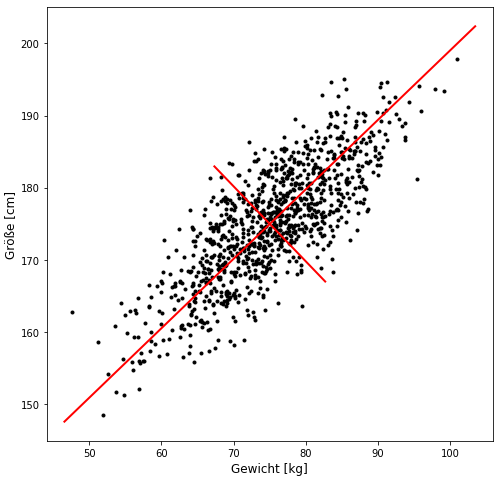
\includegraphics[width = .95\textwidth]{figures/pca_example.png}
	\caption{Simulierte Daten zu Gewicht [kg] und Größe [cm] für 1000 Personen}
	\label{pca_example_original}
	\end{subfigure}
	%	
	\begin{subfigure}{0.45\textwidth}
	\centering
	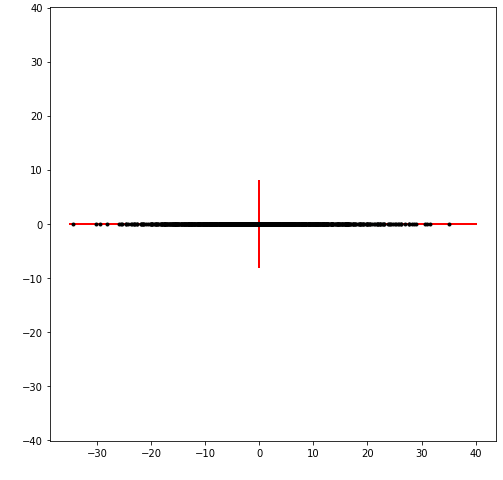
\includegraphics[width = .95\textwidth]{figures/pca_example_rotated.png}
	\caption{Daten nach der Transformation auf die erste Hauptachse}
	\label{pca_example_rotated}
	\end{subfigure}
\caption{Die Abbildung zeigt das Ergebnis einer Hauptkomponentenanalyse auf simulierten Daten. Die roten Linien stellen die beiden Hauptachsen, also die Richtungen größter Varianz des Datensatzes dar. Diese sind nach Konstruktion orthogonal.}
\label{pca_example}
\end{figure}

\subsubsection{Vorverarbeitung der Daten}

Bevor wir die Hauptkomponentenanalyse auf einen Datensatz anwenden, gibt es einen wichtigen Bearbeitungsschritt zu beachten. Wenn eine Variable weniger variiert als eine Andere aufgrund der verwendeten Einheit oder Skala kann dies zu ungewollten Ergebnissen führen. Ohne eine Vorbehandlung der Daten hat so im obigen Beispiel eine Änderung von 1cm die gleiche Bedeutung wie eine Änderung von 1kg.  Daher werden die Daten häufig einem Vorverarbeitungsschritt unterzogen. Ein zu diesem Zweck oft verwendetes Verfahren ist die Standardisierung oder auch z-Transformation genannt. Hierbei werden die Variablen $X_i$ zentriert und anschließend auf Einheitsvarianz gebracht. Dies wird erreicht, indem man $X_i$ durch $\frac{X_i - \operatorname{E}[X_i]}{\sqrt{\operatorname{Var}[X_i]}}$ ersetzt. Mathematisch gesehen wendet man das Verfahren somit auf die Stichprobenkorrelationsmatrix an.

\subsection{Maximale Varianzerhaltung}

Wir wollen nun die Intuition des minimalen Informationsverlusts mathematisch beschreiben. Gegeben sei dazu eine Matrix $\mat{X} \in \mathbb{R}^{n\times p}$, wobei $n$ die Anzahl der Beobachtungen und $p$ die Anzahl der Variablen ist. Für eine simplere Darstellung nehmen wir im Folgenden an, dass die Variablen zuvor zentriert wurden. Aufgabe der Hauptkomponentenanalyse ist es nun sukzessive Richtungen größter Varianz zu finden, die sog. \textit{Hauptachsen}. Die Koeffizienten spiegeln dabei den Beitrag jeder einzelnen Variable zur Hauptachse wider. Anschließend werden die \textit{Hauptkomponenten} definiert, welche die Darstellung der Daten bezüglich der neuen Hauptachsen sind. Wir erhalten die erste Hauptachse $\widehat{v}_1$, indem wir die Varianz entlang dieser maximieren, d.h.
\begin{align}
\label{pca_variance_maximization_first}
\widehat{v}_1 = \argmax_{\norm{v}_2 = 1} \operatorname{Var}[\mat Xv] = \argmax_{\norm{v}_2 = 1} v^T \mat{\Sigma} v
\end{align}
wobei $\mat{\Sigma} = \mat{X}^T\mat{X}$ die Stichprobenkovarianzmatrix bis auf die Bessel-Korrektur $\frac{1}{n-1}$ ist. Die restlichen Hauptachsen werden sequentiell definiert
\begin{align}
\label{pca_variance_maximization_rest}
\begin{split}
\widehat{v}_{i+1} = \argmax_{\norm{v} = 1} v^T \mat{\Sigma} v\\
\widehat{v}_{i+1}^T\widehat{v}_l = 0 \quad \forall 1 \leq l \leq i.
\end{split}
\end{align}
Man sucht also unter den Richtungen, die orthogonal zu allen bisherigen Hauptachsen sind, diejenige, die die Varianz maximiert. Durch Transformation der Daten $\widehat{Z}_i = \mat{X}\widehat{v}_i$ erhält man dann die Hauptkomponenten \cite{vidal}.

Aufgrund der schrittweisen Konstruktion gibt es eine natürliche Ordnung der Hauptkomponenten. Da keine Restriktion an die erste Hauptachse gestellt wird, erklärt die erste Hauptkomponente den größten Teil der Varianz des Datensatzes. Weitere Hauptachsen müssen orthogonal zu den Vorherigen sein und können somit nur einen geringeren Anteil erklären. Ab einem gewissen Punkt erhalten wir durch Berechnung einer weiteren Hauptkomponente also nur geringfügig mehr Information über den Datensatz. Es gilt einen Punkt der Balance zwischen erklärter Varianz und Modellkomplexität zu finden. Mit dieser Fragestellung werden wir uns weiter in Abschnitt \ref{selection_principal_components} beschäftigen.

Für die Maximierungsprobleme (\ref{pca_variance_maximization_first}) und (\ref{pca_variance_maximization_rest}) existiert eine erstaunlich einfache Lösung. Leiten wir (\ref{pca_variance_maximization_first}) in der Langrange-Form $L(v, \lambda) = v^T\mat{\Sigma}v + \lambda (1-v^Tv)$ nach $v$ ab, erhalten wir die notwendige Bedingung 
$$\frac{\partial L(v,\lambda)}{\partial v} = 2\mat{\Sigma} v -2\lambda v=0$$
und somit den stationären Punkt $\mat{\Sigma}\widehat{v}_1 = \lambda_1 \widehat{v}_1$. Das bedeutet, dass die erste Hauptachse genau dem Eigenvektor des größten Eigenwertes $\lambda_1$ der Stichprobenkovarianzmatrix $\mat \Sigma$ entspricht. Durch Linksmultiplikation mit $\widehat{v}_1^T$ sehen wir, dass durch 
$\widehat{v}_1^T\mat{\Sigma}\widehat{v}_1 = \lambda_1$ die Varianz der ersten Hauptkomponente gegeben ist. Analog zeigt man, dass auch die folgenden Hauptachsen, die durch (\ref{pca_variance_maximization_rest}) definiert sind, den Eigenvektoren von $\mat \Sigma$ entsprechen \cite{bishop}.

Daher können wir anstatt sukzessiver Berechnung einzelner Hauptachsen die Matrix $\mat{\Sigma}$ direkt diagonalisieren. Aufgrund der Symmetrie von $\mat \Sigma$ können wir eine Eigenwertzerlegung wie in Abschnitt \ref{matrix_decomposition} angeben
$$\mat{\Sigma} = \widehat{\mat V} \widehat{\mat \Lambda} \widehat{\mat{V}}^T,$$
wobei $\widehat{\mat{\Lambda}}$ eine Diagonalmatrix mit Eigenwerten $\lambda_i$ und $\widehat{\mat V}$ die Matrix der Eigenvektoren ist. Somit können die Hauptachsen direkt aus $\widehat{\mat V}$ abgelesen werden. Die Hauptkomponenten werden dann wie zuvor durch Multiplikation der Beobachtungen mit den Eigenvektoren erreicht.
$$\mat Z = \mat X \widehat{\mat V}.$$
Die $i$-te Spalte in $\mat{Z}$ entspricht also der $i$-ten Hauptkomponente und die Beobachtungen bezüglich der neuen Darstellung sind die Zeilen von $\mat{Z}$.

Es gibt einen engen Zusammenhang zwischen der Eigenwertzerlegung von $\mat X^T \mat X$ und der Singulärwertzerlegung von $\mat X$. Diese Beziehung können wir nutzen, um die Lösung noch einfacher zu gestalten. Eine Singulärwertzerlegung ergibt
$$\mat{X} = \widehat{\mat{U}}\widehat{\mat{D}}\widehat{\mat{V}}^T$$
wobei $\widehat{\mat{D}}$ die Diagonalmatrix der Singulärwerte, $\widehat{\mat{U}}$ eine orthogonale $n \times n$ und $\widehat{\mat{V}}$ eine orthogonale $p \times p$ Matrix ist. Nun sieht man aufgrund der Orthogonalität von $\widehat{\mat U}$, dass
$$\mat{\Sigma} = \mat X^T \mat X = \widehat{\mat{V}}\widehat{\mat{D}}\widehat{\mat{U}}^T \widehat{\mat{U}}\widehat{\mat{D}}\widehat{\mat{V}}^T = \widehat{\mat V} \widehat{\mat{D}}^2 \widehat{\mat V}^T.$$

Zusammengefasst können also alle relevanten Ergebnisse einer Hauptkomponentenanalyse mithilfe einer einzelnen Singulärwertzerlegung von $\mat X$ angegeben werden. Die Hauptachsen entsprechen den Eigenvektoren in $\widehat{\mat V}$, die Hauptkomponenten der Matrix $\widehat{\mat Z} = \mat X \widehat{\mat V} = \widehat{\mat U} \widehat{\mat D}$ und die zugehörigen Varianzen sind durch $\sigma_i^2$ gegeben. Für die Berechnung einer solchen Zerlegung stehen äußert effiziente Verfahren zur Verfügung, welche sowohl den $n>p$ als auch den $p>n$ Fall in $\mathcal{O}(np \cdot \min\{n,p\})$ lösen können. 

\subsection{Verbindung zur Regressionsanalyse}

Wir widmen uns nun einer anderen Sichtweise auf die Hauptkomponentenanalyse, welche einen Zusammenhang zur linearen Regression herstellt und eine geometrische Interpretation ermöglicht. Hierbei möchte man einen $k$-dimensionalen Unterraum finden, der die Daten bestmöglich approximiert. Mathematisch ausgedrückt minimieren wir also die Residuen der Projektion auf den Unterraum.

Sei dazu $x_i$ die $i$-te Beobachtung und $\mat V_k = \begin{bmatrix} v_1 & \cdots & v_k \end{bmatrix}$ eine $p \times k$ orthonormale Matrix. Wie in Abschnitt \ref{orthogonality} beschrieben, wird durch den Operator $\mat V_k \mat V_k^T$ jede Beobachtung orthogonal auf den durch $v_1, \ldots , v_k$ aufgespannten Unterraum projiziert. Eine bestmögliche $\ell_2$-Approximation der Daten ist gegeben, wenn wir die Distanz zwischen jeder Beobachtung und seiner Projektion minimieren \cite{zou_sparsepca}:
\begin{align}
\label{pca_regression_formulation}
\begin{split}
\mat{\widehat{V}}_k = \argmin_{\mat{V}_k} \sum_{i=1}^{n} \norm{x_i - \mat{V}_k \mat{V}_k^Tx_i}_2^2\\
\mat{V}_k^T\mat{V}_k = I_{k \times k}
\end{split}
\end{align}
Ein mathematisch rigoroser Beweis, dass die Lösung von (\ref{pca_regression_formulation}) genau den ersten $k$ Hauptachsen entspricht, befindet sich in \cite{vidal}. Wir möchten hier eine intuitive Erklärung für diese Äquivalenz geben. Sprechen wir von der Varianz eines Datensatzes, meinen wir die Summe der Varianzen der einzelnen Variablen. Somit ist die Gesamtvarianz durch $\norm{\mat X}_{F}^{2}$ gegeben. Aufgrund der orthogonalen Projektion erhalten wir mithilfe des verallgemeinerten Satzes von Pythagoras
\begin{align*}
\norm{\mat X}_{F}^{2} & = \sum_{i=1}^{n} \norm{x_i}_{2}^{2}\\
& = \sum_{i=1}^{n} \norm{x_i - \mat V_k \mat V_k^T x_i + \mat V_k \mat V_k^T x_i}_{2}^{2}\\
& = \sum_{i=1}^{n} \norm{x_i - \mat V_k \mat V_k^T x_i}_2^2 + \norm{\mat V_k \mat V_k^T x_i}_{2}^{2}\\
& = \norm{\mat X - \mat X \mat V_k \mat V_k^T}_{F}^{2} + \norm{\mat X \mat V_k \mat V_k^T}_{F}^{2}.
\end{align*}
Weiter sehen wir, dass
\begin{align*}
\norm{\mat X \mat V_k \mat V_k^T}_{F}^{2} & = \spur{\mat X \mat V_k \mat V_k^T (\mat X \mat V_k \mat V_k^T)^T}\\
& = \spur{\mat V_k^T \mat X^T \mat X \mat V_k}\\
& = \sum_{i=1}^{k} v_i^T (\mat X^T \mat X) v_i
\end{align*}
und somit
\begin{align*}
\norm{\mat X}_{F}^{2} = \norm{\mat X - \mat X \mat V_k \mat V_k^T}_{F}^{2} + \sum_{i=1}^{k} v_i^T (\mat X^T \mat X) v_i.
\end{align*} 
Nun sind wir in der Lage, die Verbindung zur ursprünglichen Konstruktion in (\ref{pca_variance_maximization_first}) und (\ref{pca_variance_maximization_rest}) zu sehen. Dort haben wir den Term $v_i^T (\mat X^T \mat X) v_i$, der die Varianz der $i$-ten Hauptkomponente beschreibt, sequentiell maximiert. Mathematisch gesehen macht es keinen Unterschied, ob wir die Varianz der Hauptkomponenten $\sum_{i=1}^{k} v_i^T (\mat X^T \mat X) v_i$ maximieren oder die Residuen der Projektion $\norm{\mat X - \mat X \mat V_k \mat V_k^T}_{F}^{2}$ minimieren. Diese Idee ist in Abbildung \ref{pca_projection_explanation} geometrisch veranschaulicht. Im linken Bild versucht man eine Richtung durch den Datensatz zu finden, welche die Varianz entlang dieser maximiert. Im Gegensatz dazu sucht man im rechtem Bild nach einer Richtung, welche die Summe der Distanzen zwischen Datenpunkt und seiner Projektion minimiert. In beiden Fällen resultiert dieselbe Hauptachse.

\begin{figure}
\centering
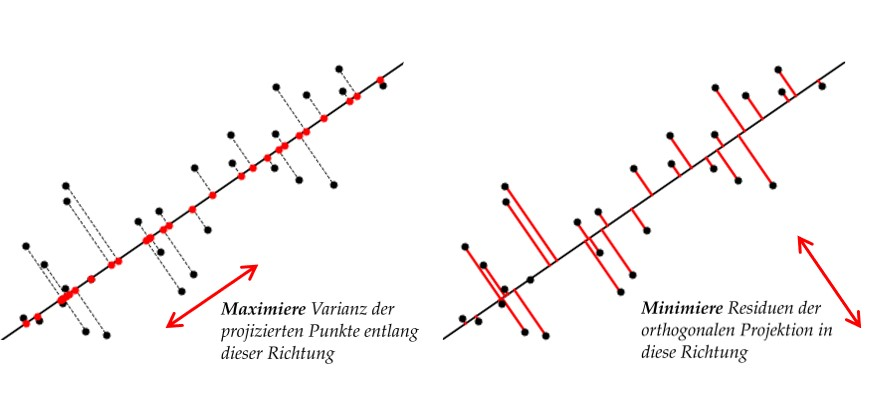
\includegraphics[width = 0.9\textwidth]{figures/pca_projection_explanation.jpg}
\caption{Die Abbildung zeigt die Äquivalenz von Maximierung der Varianz und Minimierung der Residuen in zwei Dimensionen.}
\label{pca_projection_explanation}
\end{figure} 

%Drücken wir (\ref{pca_variance_maximization_first}) und (\ref{pca_variance_maximization_rest}) in einem gemeinsamen Berechnungsproblem aus ergibt sich
%\begin{align}
%\label{pca_variance_maximization}
%\begin{split}
%\widehat{\mat V}_k = \argmax_{\mat V_k}\sum_{i=1}^{k} v_i^T \mat \Sigma v_i\\
%\mat V_k^T\mat V_k = \mat I_{k \times k}
%\end{split}
%\end{align}

Da die Daten auf den niedrigdimensionaleren Raum linear transformiert werden, gehört die Hauptkomponentenanalyse zu den linearen Dimensionsreduktionsverfahren. Anhand von (\ref{pca_regression_formulation}) erkennt man zudem einen starken Zusammenhang zur linearen Regression, bei welcher ebenfalls die Summe der Residuenquadrate minimiert werden. Neben der abweichenden Motivation der beiden Verfahren liegt der entscheidende Unterschied in der Art der Projektion. Während bei linearer Regression die Projektion orthogonal bezüglich der unabhängigen Koordinatenachsen ist, werden die Daten bei der Hauptkomponentenanalyse orthogonal auf die Hauptachsen projiziert. Ausgehend von (\ref{pca_regression_formulation}) werden wir in Kapitel \ref{sparse_pca} die Variante der dünnbesetzten Hauptkomponentenanalyse beschreiben.

\subsection{Weitere Formulierungen} 

Wir werden nun kurz auf zwei weitere Formulierungen eingehen, anhand welcher weitere Eigenschaften der Hauptkomponentenanalyse deutlich werden. Ersetzt man in (\ref{pca_regression_formulation}) $\mat X \widehat{\mat V}_k^T$ durch die Hauptkomponenten $\widehat{\mat Z}_k$ erhält man
\begin{align}
\label{pca_minimize_reconstruction_error}
\begin{split}
(\widehat{\mat{Z}}_k, \widehat{\mat V}_k) = \argmin_{\mat Z_k, \mat V_k} \norm{\mat X - \mat Z_k \mat V_k^T}_{F}^{2}\\
\mat V_k^T\mat V_k = \mat I_{k \times k}.
\end{split}
\end{align}
Durch $\widehat{\mat Z}_k \widehat{\mat V}_k^T$ ist eine bestmögliche Rekonstruktion der Datenmatrix $\mat X$ gegeben. In anderen Worten wird in (\ref{pca_minimize_reconstruction_error}) also der $\ell_2$-Rekonstruktionsfehler minimiert. Diese Formulierung wird häufig für Verallgemeinerungen der Hauptkomponentenanalyse gewählt und werden wir in Abschnitt \ref{adjustment_of_variances} gebrauchen.

Für eine letzte Formulierung erinnern wir uns, dass die abgeschnittene Singulärwertzerlegung $\widehat{\mat X}_k = \widehat{\mat U}_k \widehat{\mat D}_k \widehat{\mat{V}}_k^T \in \mathbb{R}^{n \times k}$ die optimale Lösung für die Hauptkomponentenanalyse liefert. Diese ist aufgrund des Eckart-Young-Mirsky-Theorem aus Abschnitt \ref{matrix_approximation} ebenfalls Lösung des Problems
\begin{align}
\label{pca_best_rank_approximation}
\begin{split}
\widehat{\mat X}_k = \argmin_{\mat X_k} \norm{\mat X - \mat X_k}_F^2\\
\rang{\mat X_k} \leq k.
\end{split}
\end{align}
Somit ist $\widehat{\mat X}_k$ diejenige Matrix mit Rang $k$, die $\mat X$ am Besten approximiert. Mithilfe des Theorems können wir den Fehler, der durch die Dimensionsreduktion entsteht, explizit angeben
\begin{align*}
\norm{\mat X - \widehat{\mat X}_k}_F^2 = \sum_{i=k+1}^p \sigma_i^2.
\end{align*}
Infolgedessen können wir Bewertungskriterien definieren, welche es uns ermöglichen, verschiedene Modelle miteinander zu vergleichen. Wir wollen uns nun mit der Frage beschäftigen, wie stark wir die Dimension eines Datensatzes reduzieren können.


%----------------------------------------------------------------------------------------
%	Selektion der Hauptkomponenten
%----------------------------------------------------------------------------------------


\section{Selektion der Hauptkomponenten}
\label{selection_principal_components}

Optimale Hyperparameter für ein Modell zu finden ist selten einfach. Auch bei Dimensionsreduktionsverfahren kennen wir oft die intrinsische Dimension unserer Daten a priori nicht. Daher ist es schwer zu sagen, wie viele Hauptkomponenten benötigt werden, um die Daten passend zu modellieren. Es gilt einen Punkt der Balance zwischen Rekonstruktionsfehler und Modellkomplexität zu finden, welcher vom Anwendungsfall abhängen kann. Als Maß für die Modellkomplexität eignet sich aufgrund der natürlichen Ordnung in diesem Fall die Anzahl an Hauptkomponenten $k$ bzw. der Rang von $\widehat{\mat X}_k$. Arbeiten wir auf rauschfreien Daten können wir $k$ durch $\rang{\mat X}$ schätzen. In der Regel ist unser Datensatz aber durch Rauschen gestört, weshalb $\mat X$ vollen Rang hat.

Aufgrund der Effizienz der Singulärwertzerlegung berechnet man häufig zunächst alle $k \leq \min\{n, p\}$ Hauptkomponenten. Die eigentliche Dimensionsreduktion findet dann durch Selektion statt. Bewertet werden die verschiedenen Modelle mithilfe des Rekonstruktionsfehlers bzw. der erklärten Varianz $\sigma_i^2$ der einzelnen Hauptkomponenten. So können wir $k$ zum Beispiel so wählen, dass der Rekonstruktionsfehler durch einen Parameter $\tau$ beschränkt ist
\begin{align}
\label{pca_model_selection}
\widehat{k} = \min_k \left\{k \colon \sum_{i = k+1}^{p} \sigma_i^2 < \tau \right\} \quad \text{oder} \quad \widehat{k} = \min_k \left\{k \colon \sigma_{k+1}^2 < \tau \right\}.
\end{align}
Das zweite Auswahlkriterium wird in Abbildung \ref{scree_plot} veranschaulicht. In der Praxis ist es aber sehr schwer, $\tau$ angemessen zu wählen, da die Singulärwerte von $\mat X$ nicht invariant unter Skalierung sind. Daher werden die Singulärwerte meist normiert
\begin{align}
\label{pca_model_selection_normed}
\widehat{k} = \min_k \left\{k \colon \frac{\sum_{i = k+1}^{p} \sigma_i^2}{\sum_{i=1}^k \sigma_i^2} < \tau \right\} \quad \text{oder} \quad \widehat{k} = \min_k \left\{k \colon \frac{\sigma_{k+1}^2}{\sum_{i=1}^k \sigma_i^2} < \tau \right\}.
\end{align}
Ersteres Auswahlkriterium in (\ref{pca_model_selection_normed}) ist weit verbreitet. Man wählt genau so viele Hauptkomponenten aus, dass höchstens ein gewisser Anteil der Varianz verloren geht. Typische Werte für $\tau$ liegen zwischen 10\% und 20\%. 

In manchen Fällen gibt es eine klare Trennung in der Größe der Singulärwerte. Vidal et al. \cite{vidal} definieren ein Kriterium
\begin{align}
\widehat{k} = \argmin_{k} \quad \alpha\sigma_{k+1}^2 + \beta k,
\end{align}
welches im Wesentlichen nach einem starken Einbruch der Singulärwerte sucht. Mit $\alpha, \beta > 0$ haben wir damit direkten Einfluss auf das Verhältnis zwischen Rekonstruktionsfehler und Modellkomplexität. In Abbildung \ref{scree_plot} haben wir die resultierende Gerade eingezeichnet.

\begin{figure}
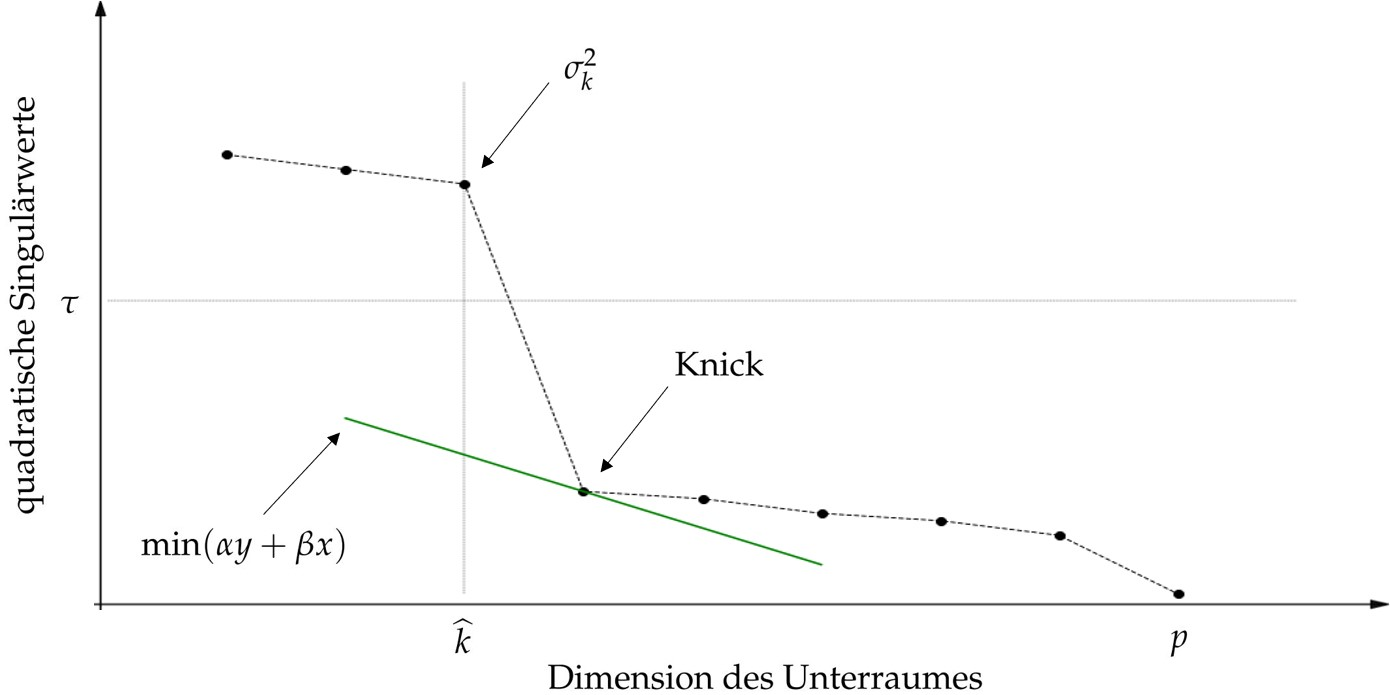
\includegraphics[width=0.9\textwidth]{figures/scree_plot_explanation.jpg}
\caption{Die Abbildung zeigt einen sog. \textit{Scree Plot}, welche die quadratischen Singulärwerte bzw. die erklärte Varianz jeder einzelnen Hauptkomponente zeigt. Die Darstellung wird häufig genutzt, um zu entscheiden wie viele Hauptkomponenten für ein geeignetes Modell auszuwählen sind. (Abbildung basiert auf \cite{vidal})}
\label{scree_plot}
\end{figure}

In der Literatur existieren weitere Heuristiken, auf die wir hier nicht näher eingehen werden. Bis vor Kurzem gab es keinerlei theoretische Resultate für die Modellwahl bei der Hauptkomponentenanalyse. Gavish und Donoho \cite{gavish} haben erstmals ein optimales Kriterium im asymptotischem Fall angeben können, welche der Singulärwerte beibehalten werden sollten. Unter der Annahme, dass das Signal-Rausch-Verhältnis konstant bleibt, zeigen sie, dass der asymptotische mittlere quadratische Fehler 
$$\operatorname{AMSE} = \lim_{n \rightarrow \infty} \norm{\mat X - \widehat{\mat X}_k}_{F}^{2}$$
für $n \times n$-Matrizen minimal wird, falls alle Singulärwerte kleiner als $\frac{4}{\sqrt{3}}\sqrt{n}\sigma \approx 2.309\omega$ auf Null gesetzt werden. Wenn die Stärke des Rauschens $\omega$ vorher nicht bekannt ist, ändert sich die Schranke zu $2.858\omega_{med}$, wobei $\omega_{med}$ der Stichprobenmedian der Singulärwerte ist. Für nicht quadratische $m \times n$-Matrizen ändern sich die Schwellenwerte abhängig von $m,n$. Auch wenn damit nur ein asymptotisches Resultat zur Verfügung steht, scheint diese Schranke in der Praxis hilfreich zu sein.


%----------------------------------------------------------------------------------------
%	Grenzen der Anwendbarkeit
%----------------------------------------------------------------------------------------


\section{Grenzen der Anwendbarkeit} \label{theo_results}

Obwohl die Hauptkomponentenanalyse in vielen Situationen helfen kann, Datensätze zu veranschaulichen und zu strukturieren, gibt es keine Garantie für sinnvolle Ergebnisse. Im Folgendem werden wir Szenarien beschreiben, bei denen unerwünschte Effekte bei der Verwendung dieses Verfahrens auftreten. Daher gilt es den Datensatz vorerst hinsichtlich folgender Gesichtspunkte zu untersuchen: 

\begin{itemize}
\item Existenz linearer Beziehungen zwischen Variablen
\item Vollständigkeit des Datensatzes
\item Ausreißer in den Daten
\item Anzahl an Beobachtungen in Relation zu Anzahl an Variablen
\end{itemize}

Bei der Hauptkomponentenanalyse können lineare Korrelationen zwischen Variablen sehr gut eingefangen werden. Andere Beziehungen, die durchaus in der Praxis vorkommen, werden dabei nicht berücksichtigt bzw. als linear angenommen. Vidal et al. \cite{vidal} zeigen am Beispiel von Porträt-Fotos auf, dass nichtlineare Strukturen in der Tat verloren gehen. In manchen Fällen können wir mithilfe geeigneter Koordinatentransformationen dieses Hindernis umgehen. Bei der Anwendung des sog. \textit{Kernel Tricks} transformiert man die Daten in einen höherdimensionalen Raum, in welchem sie besser linear separierbar sind. \textit{Kernel PCA} wendet die Hauptkomponentenanalyse in diesem Raum an bevor die Daten wieder zurück transformiert werden. Andere Erweiterungen, die unter der Kategorie \textit{manifold learning} zusammengefasst werden können, versuchen die lokale Geometrie der Mannigfaltigkeit direkt zu approximieren. So kann man ohne die Nutzung eines höherdimensionalen Raumes unmittelbar die niedrigdimensionale Struktur erhalten. Verfahren, die diesen Ansatz verfolgen, sind zum Beispiel die \textit{multidimensionale Skalierung} oder \textit{ISOMAP} \cite{lee}.

Falls wir einen unvollständigen Datensatz vorliegen haben, bei welchem manche Werte korrupt oder nicht vorhanden sind, können wir die klassische Hauptkomponentenanalyse nicht anwenden. Falls dies nur einen Bruchteil der Daten betrifft, können durch entsprechende Erweiterungen mit hoher Wahrscheinlichkeit noch immer exakte Ergebnisse erzielt werden \cite{candes}. Des Weiteren ist das Verfahren sehr sensitiv gegenüber Ausreißern. Besonders wenn nur wenige Beobachtungen zur Verfügung stehen, können Ausreißer die Resultate drastisch beeinflussen. Um eine Verfälschung der Ergebnisse zu vermeiden, entfernt man diese meist vor der Anwendung. Allerdings ist es nicht immer einfach Ausreißer zu identifizieren. Daher wird in \cite{kriegel} vorgeschlagen, die Datenpunkte vorab unterschiedlich zu gewichten basierend auf deren geschätzten Relevanz. Die Behandlung dieser Art Probleme wird mit dem Begriff \textit{Robust PCA} verbunden.

Viele gegenwärtige Datensätze besitzen eine vergleichsweise hohe Anzahl an Variablen im Vergleich zur Anzahl an Beobachtungen. Typische Anwendungsgebiete sind die Bildbearbeitung, Signal- oder  Genexpressionsanalyse, in welchen viele Variablen in Form von Pixeln, Frequenzen oder Genen vorkommen. Auch wir werden uns in Kapitel \ref{application} mit einem Datensatz dieser Art beschäftigen. In Theorem \ref{pca_inconsistency_ratio} werden wir sehen, dass es in einer solchen Situation zur \textit{Inkonsistenz} der Hauptkomponentenanalyse kommen kann. Deswegen muss in diesen Fällen genau überprüft werden, ob den Ergebnissen getraut werden kann.

Das wohl wichtigste Hindernis im Zuge dieser Arbeit sind sicherlich die durch die Transformation entstehenden Interpretationsschwierigkeiten. Da jede Hauptkomponente durch eine Linearkombination aller Ausgangsvariablen entsteht, ist es in hochdimensionalen Fällen fast unmöglich diesen eine Bedeutung im Kontext zuzuweisen. Dieser Interpretationsverlust ist Ausgangspunkt der Idee der \textit{dünnbesetzten Hauptkomponentenanalyse (kurz: {Sparse PCA})}, welchem das folgende Kapitel \ref{sparse_pca} gewidmet ist.


%----------------------------------------------------------------------------------------
%	Erweiterungen der Hauptkomponentenanalyse
%----------------------------------------------------------------------------------------


%\section{Erweiterungen der Hauptkomponentenanalyse}
%\label{pca_extensions}
%
%\begin{table}
%\centering
%\begin{tabular}[c]{lll}
%\thead{Verlustfunktion} & \thead{Regularisierung} & \thead{Nebenbedingung}\\
%\hline \rule{0pt}{1.5\normalbaselineskip}
%\makecell{quadratisch\\(reelle Daten)} & \makecell{$\ell_2$-Norm\\(kleine Koeffizienten)} & \makecell{orthogonal\\(orthogonale Hauptachsen)}\vspace{0.25cm}\\
%\makecell{absolut\\(robust gegenüber\\Ausreißern)} & \makecell{$\ell_1$-Norm\\(dünnbesetzte Koeffizienten)} & \makecell{nichtnegativ\\(nichtnegative Koeffizienten)}\vspace{0.25cm}\\
%\makecell{logistisch\\(Binärdaten)} & \makecell{Ableitung\\ (glatte Koeffizienten)}\vspace{0.25cm}\\
%\end{tabular}
%\caption{Zusammenfassung einiger Erweiterungen der Hauptkomponentenanalyse in einem konsistenten Schema.}
%\label{pca_extensions_overview}
%\end{table}
%
%Im vorangegangenem Abschnitt haben wir bereits auf Erweiterungen der Hauptkomponentenanalyse hingewiesen, welche Grenzen der klassischen Variante überkommen. Viele dieser können mithilfe eines allgemeinen Schemas formuliert werden
%\begin{align}
%\begin{split}
%\argmin_{\mat{Z},\mat{V}} \underbrace{L(\mat{Z}, \mat{V})}_{\text{Verlustfunktion}} + \underbrace{\lambda_z f_z(\mat Z) + \lambda_v f_v(\mat V)}_{\text{Regularisierung}}\\
%\text{unter der Nebenbedingung, dass} \quad \underbrace{\mat Z \in \Omega_z, \mat V \in \Omega_v}_{\text{Nebenbedingung}}.
%\end{split}
%\end{align}
%In Tabelle \ref{pca_extensions_overview} sind einige Ideen, die in der Literatur betrachtet werden, festgehalten. Dabei können Verlustfunktion, Regularisierung und Nebenbedingungen beliebig kombiniert werden, um ein für den Anwendungsfall geeignetes Modell zu erstellen.


%----------------------------------------------------------------------------------------
%	Theoretische Aussagen
%----------------------------------------------------------------------------------------


\section{Theoretische Aussagen}
\label{pca_theorems}

Zu Abschluss dieses Kapitels werden wir interessante Eigenschaften sowie Theoreme präsentieren. Der Fokus wird vor allem auf der Inkonsistenz der Hauptkomponentenanalyse in hochdimensionalen Fällen liegen.

Eine wichtige Eigenschaft ist die Unkorreliertheit der Hauptkomponenten. Dies lässt sich anhand der Stichprobenkovarianzmatrix der Hauptkomponenten $\hat{\mat Z}^T \hat{\mat Z} = (\mat X \hat{\mat V})^{\top}\mat X \hat{\mat V} = \hat{\mat V}^{\top}\mat{\Sigma}\hat{\mat V}$ sehen, welche aufgrund von $\hat{\mat V}^T \hat{\mat V} = \mat I_{k \times k}$ eine Diagonalmatrix ist. Somit können wir von einer Hauptkomponente und deren erklärte Varianz sprechen, ohne uns dabei auf andere beziehen zu müssen.

Für unseren Anwendungsfall in Kapitel \ref{application} befinden wir uns in einem $p \gg n$ Szenario. Es gibt eine Reihe theoretischer Aussagen, welche eine Inkonsistenz im asymptotischem Fall zeigen. Asymptotische Studien der Hauptkomponentenanalyse fallen in verschiedene Kategorien abhängig vom Verhältnis zwischen $n$ und $p$.
\begin{itemize}
\item In der klassischen Asymptotik untersucht man die Effekte für $n \rightarrow \infty$ mit fixierter Dimension $p$.
\item In der Theorie der Zufallsmatrizen erhöhen wir sowohl $n$ als auch $p$ mit der Voraussetzung, dass das Verhältnis $\frac{p_n}{n}$ asymptotisch konstant ist.
\item In einem \textit{high dimension low sample size setting (HDLSS)} betrachten wir die Asymptotik für $p \rightarrow \infty$ mit fixierter Anzahl an Beobachtungen $n$.
\end{itemize}
Zunächst gilt es den Begriff der \textit{Inkonsistenz} in Bezug auf die Hauptkomponentenanalyse genauer zu verstehen. In dieser Arbeit haben wir eine Stichprobenversion der Hauptkomponentenanalyse eingeführt. Indem man die Stichprobenkovarianzmatrix $\mat\Sigma$ durch die Kovarianzmatrix in (\ref{pca_variance_maximization_first}) ersetzt, erhält man eine Populationsversion der Hauptkomponentenanalyse. Unter der Annahme, dass die gegebenen Daten ein endliche, zufällige Stichprobe einer meist unbekannten Verteilung sind, stellt sich die Frage in welcher Relation die Ergebnisse stehen. Genauer gesagt interessiert man sich dafür, ob die Hauptachsen der Stichproben- und der Populationsversion identisch sind. Um die Hauptachsen miteinander zu vergleichen beziehen wir uns auf den Winkel zwischen Beiden.

\begin{defn}[Konsistenz \cite{shen_consistency}]
Die Stichprobenhauptachse $\hat{v}_i$ ist mit der Populationshauptachse $v_i$
\begin{itemize}
\item \textit{konsistent}, falls $\operatorname{angle}(\widehat{v}_i, v_i) \longrightarrow 0$
\item \textit{marginal inkonsistent}, falls $\operatorname{angle}(\widehat{v}_i, v_i) \longrightarrow c \in (0,\frac{\pi}{2})$
\item \textit{stark inkonsistent}, falls $\operatorname{angle}(\widehat{v}_i, v_i) \longrightarrow \frac{\pi}{2}$
\end{itemize} 
für $n \to \infty$ bzw. $p \rightarrow \infty$. 
\end{defn}

Abhängig von $n$, $p$ und der Stärke des Rauschens im Modell ergeben sich unterschiedliche Ergebnisse für die Konsistenz der Hauptkomponentenanalyse. Allgemein ist die Tendenz, dass eine hohe Anzahl an Beobachtungen die Konsistenz der Hauptachsen fördert, während eine erhöhte Dimension eine Inkonsistenz hervorruft. Nicht überraschend kann man zeigen, dass die Eigenvektoren der Stichprobenkovarianzmatrix $\widehat{v}_i$ konsistente Schätzer für die Eigenvektoren der Kovarianzmatrix $v_i$ sind, falls wir die Dimension fixieren und die Anzahl an Beobachtungen erhöhen $n \rightarrow \infty$ \cite{anderson}. Für unser Szenario jedoch interessanter sind hochdimensionale Fälle. Weil eine Betrachtung einer HDLSS-Situation die Einführung zu vieler neuer Prinzipien erfordern würde, präsentieren wir zum Abschluss dieses Kapitels ein Inkonsistenz-Theorem für den Fall eines asymptotisch konstanten Verhältnisses zwischen $n$ und $p$. Dafür betrachten wir ein \textit{single component model} \cite{johnstone}
\begin{align}
\label{single_component_model}
x_i = l_i v_1 + \sigma r_i \quad i = 1, \ldots n,
\end{align}
in welchem $v_1 \in \mathbb{R}^p$ der zu schätzende Eigenvektor ist. Dabei sind $l_i \sim N(0,1)$ unabhängig gleichverteilte Gaußsche Zufallseffekte und $r_i \sim N_p(0, \mat I)$ unabhängige Rauschvektoren. Wegen der Rauscheffekte hat die Stichprobenkovarianzmatrix $\mat\Sigma$ fast sicher $\min\{n,p\}$ von null verschiedene Eigenvektoren. Sei $\widehat{v}_1$ der größte Stichprobeneigenvektor von $\mat \Sigma$. Mit dem folgendem Theorem haben wir eine notwendige und hinreichende Bedingung für die Konsistenz der ersten Stichprobenhauptachse.

\begin{thm}[Inkonsistenz der Hauptkomponentenanalyse bei konstantem asymptotischem Verhältnis von $n$ und $p$ \cite{johnstone}]
\label{pca_inconsistency_ratio}
Sei $\sigma$ die Stärke des Rauschens im Modell (\ref{single_component_model}) und $\lim_{n \rightarrow \infty} \frac{\norm{v_1}^{2}}{\sigma^2} = \omega > 0$ das limitierende Signal-Rausch-Verhältnis. Weiterhin sei 
$$R(\widehat{v}_1, v_1) = \inner{\frac{\widehat{v}_1}{\norm{\widehat{v}_1}}}{\frac{v_1}{\norm{v_1}}} = \cos{(\operatorname{angle}(\widehat{v}_1, v_1))}.$$
Unter der Annahme, dass $\lim_{n \rightarrow \infty} \frac{p_n}{n} = c$ gilt
$$\mathbb{P}\left[\lim_{n \rightarrow \infty} R^2(\widehat{v}_1, v_1) = R_{\infty}^2(\omega, c)\right] = 1$$
wobei $R_{\infty}^2(\omega, c) = \frac{(\omega^2 - c)_+}{\omega^2 + c\omega}$.
\end{thm}

Wir sehen, dass $R_{\infty}^2(\omega, c) < 1$ genau dann, wenn $c > 0$. Daher ist $\widehat{v}_1$ genau dann ein konsistenter Schätzer für $v_1$, wenn $c = 0$. Für $c > 0$ ist die Hauptkomponentenanalyse somit inkonsistent. 

Ein sehr ähnliches Resultat hält auch für ein sog. \textit{spiked covariance model}, in welcher mehrere Komponenten betrachtet werden \cite{paul}. Des Weiteren zeigen Jung und Marron eine starke Inkonsistenz der Stichprobenhauptachsen in einer HDLSS-Situation unter geeigneten Modellannahmen. In diesem Fall kann Konsistenz nur dann gewährleistet werden, wenn es eine deutliche Trennung in der Größe der Eigenwerte gibt. Für Details weiterer spezieller Bedingungen verweisen wir auf \cite{jung}.

